% !TEX options=--shell-escape
	\documentclass{article}
	\usepackage{amsmath,amssymb}
	\usepackage[inline]{enumitem}
	\usepackage{blindtext}
	\usepackage{booktabs}
	\usepackage{graphicx}
	\usepackage{xcolor}
	\usepackage[vmargin = 1.5in, top = 1in, bottom = 1.2in, letterpaper]{geometry}
	\usepackage{listings}
	\usepackage{courier}
	\usepackage{multicol}
	\usepackage{multirow}
	\usepackage{bm}
	\usepackage[labelformat=simple]{subcaption}
	\renewcommand\thesubfigure{(\alph{subfigure})}
	\usepackage{minted}
	\usepackage{fvextra}
	\definecolor{bg}{rgb}{0.95,0.95,0.95}
	\newminted{r}{mathescape, breaklines, linenos = true, bgcolor = bg, fontsize = \footnotesize}
	\usemintedstyle{tango}
	% \lstset{
	% basicstyle = \small\tt,
	% keywordstyle = \tt\color{blue},
	% commentstyle = \it\color[cmyk]{1,0,1,0},
	% stringstyle = \tt\color[RGB]{128,0,0},
	% %frame = single,
	% backgroundcolor = \color[RGB]{245,245,244},
	% breaklines,
	% extendedchars = false,
	% xleftmargin = 2em,
	% xrightmargin = 2em,
	% aboveskip = 1em,
	% tabsize = 4,
	% showspaces = false
	% }
	\newcommand\inner[2]{\left\langle{#1},{#2}\right\rangle}
	\DeclareMathOperator{\Corr}{Corr}
	\DeclareMathOperator{\Cov}{Cov}
	\DeclareMathOperator{\Var}{Var}
	\DeclareMathOperator{\E}{E}



	\begin{document}
	
	% \newfontfamily\courier{Courier New}

	
	\title{STAT 501 Exam 2}
	\author{Yifan Zhu}
	\maketitle
	
	\begin{enumerate}[leftmargin = 0 em, label = \arabic*., font = \bfseries]
	\item
	We check multivariate normality for each of the 3 cultivars using \verb|testnormality| and \verb|mvnorm.etest|.
	\begin{rcode}
# read data
wine <- read.table("wine.dat", head = F, sep = ",",
                   col.names = c("Cultivar","Alcohol", "Malic acid", "Ash", "Alkalinity of ash",
                                 "Magnesium", "Total phenols", "Flavanoids", "Nonflavanoid phenols",
                                 "Proanthocyanins", "Color intensity", "Hue", "OD280/OD315", "Proline"))
wine$Cultivar <- as.factor(wine$Cultivar)
# check multivariate normality for each cultivar
source("testnormality.R")
library(energy)
library(dplyr)
wine %>% group_by(Cultivar) %>% do(data.frame(testnormality = testnormality(.[,-1]), 
                                          energytest = mvnorm.etest(.[,-1], R = 999)$p.value))
	\end{rcode}

	The result is shown in a table, each row is a group and the \verb|testnormality| and \verb|energytest| are p-values of the tests.
	\begin{rcode}
  Cultivar testnormality energytest
  <fct>            <dbl>      <dbl>
1 1          0.656           0.0280
2 2          0.000000712     0.    
3 3          0.794           0.456 
	\end{rcode}
	From the result we can see, the p-values from both tests for Cultivar 3 are large, thus we conclude the multivariate normality holds for Cultivar 3. The p-values from both tests are small for Cultivar 2, and we reject the bull hypothesis and conclude that the mulivariate normality does not hold for Cultivar 2. For Cultivar 1, the p-values from \verb|testnormality| is large, while the p-value from \verb|energytest| is small. But since the p-value from \verb|testnormality| is pretty big, we still conclude that multivariate normality holds for Cultivar 1.

	\item 
	Before doing the clustering, we first standardize the data.
	\begin{rcode}
# cultivar information
cultivar <- wine$Cultivar

# standardize data
wine.sc <- scale(wine[,-1])
	\end{rcode}
	\begin{enumerate}
		\item 
		Hierarchical clustering with average linkage:

		The hierarchical tree is shown in Figure~\ref{tree}. Then we take number of group to be 3 and display the clustering result using \verb|ggandrews| in Figure~\ref{hc}.
		\begin{rcode}
source("ggandrews.R")
# Hierarchical clustering with average linkage
hc <- hclust(dist(wine.sc), method = "average")
plot(hc, main = "")

# display using ggandrews
ggandrews(data.frame(cutree(hc, k = 3), wine.sc), clr = 1, return_value = F)
		\end{rcode}

		\begin{figure}[!htb]
			\centering
			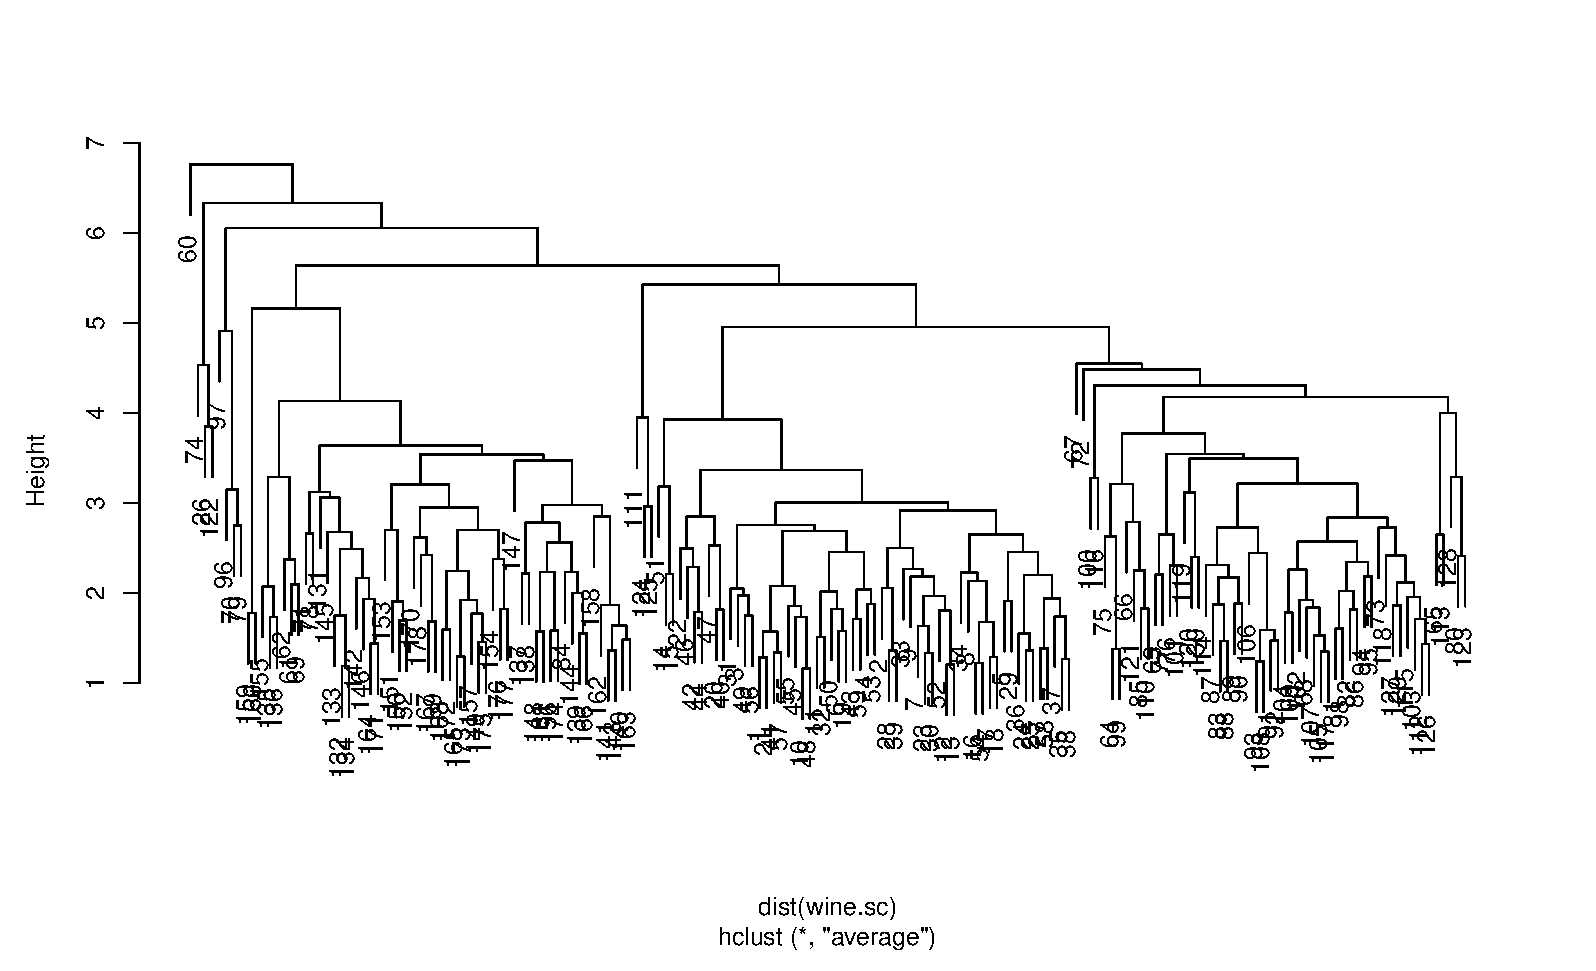
\includegraphics[width = 0.7\textwidth]{tree.eps}
			\caption{Hierarchical clustering tree}
			\label{tree}
		\end{figure}

		\begin{figure}[!htb]
			\centering
			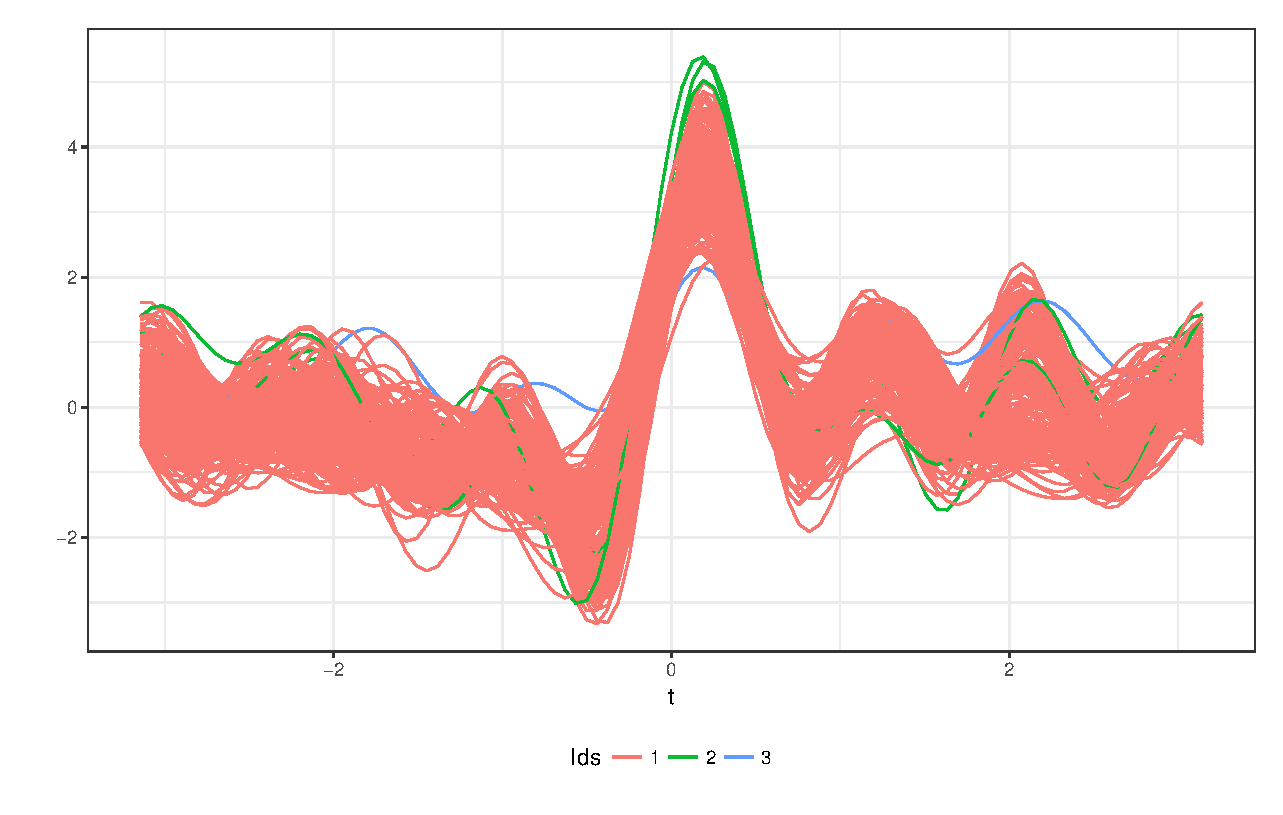
\includegraphics[width = 0.7\textwidth]{hc.eps}
			\caption{Hierarchical clustering with average linkage result, $K = 3$}
			\label{hc}
		\end{figure}

		\item 
		K-means clustering:

		Here we use 2 different initializations. One is using the result from hierarchical clustering with average linkage in (a), another is random initialization. The results are displayed using \verb|ggandrews| in Figure~\ref{km} and Figure~\ref{kmr}.
		\begin{rcode}
# k-means initialized with hc
kmnsinithcl <- function(x.data, nclus, ncut = nclus, hcl.tree)
{
  x.hcl <- hcl.tree
  x.cl <- cutree(x.hcl, k = ncut)
  data.x <- data.frame(x.data, cl = x.cl)
  means <- aggregate(. ~ cl, data = data.x, FUN = mean)
  return(kmeans(x.data,centers= means[, -1]))
}

km <- kmnsinithcl(wine.sc, nclus = 3, ncut = 3, hcl.tree = hc)

# display using ggandrews
ggandrews(data.frame(km$cluster, wine.sc), clr = 1, return_value = F)

# k-means with random initialization
km.r <- kmeans(wine.sc, centers = 3, nstart = 10000)

# display using ggandrews
ggandrews(data.frame(km.r$cluster, wine.sc), clr = 1, return_value = F)
		\end{rcode}

		\begin{figure}[!htb]
			\centering
			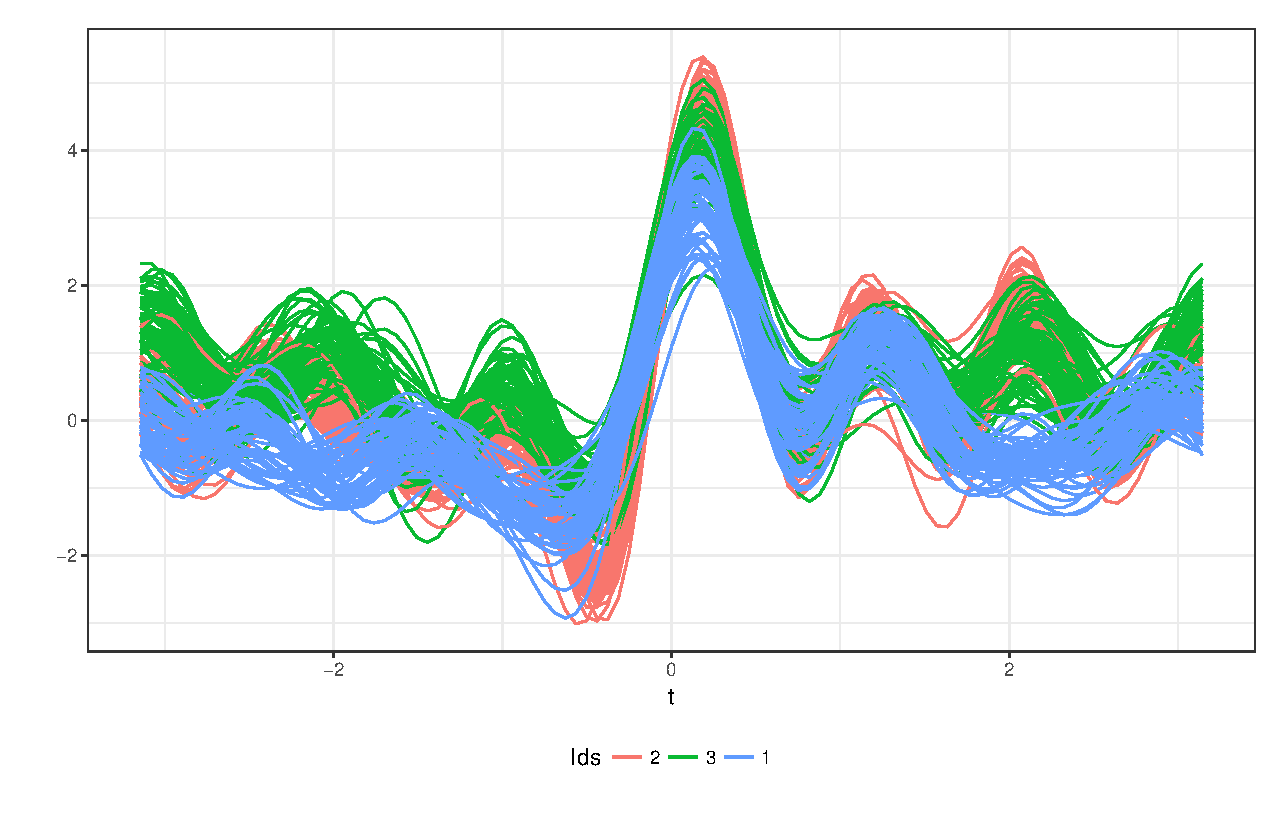
\includegraphics[width = 0.7\textwidth]{km.eps}
			\caption{K-means clustering result initialized with hierarchical clustering result, K = 3}
			\label{km}
		\end{figure}

		\begin{figure}[!htb]
			\centering
			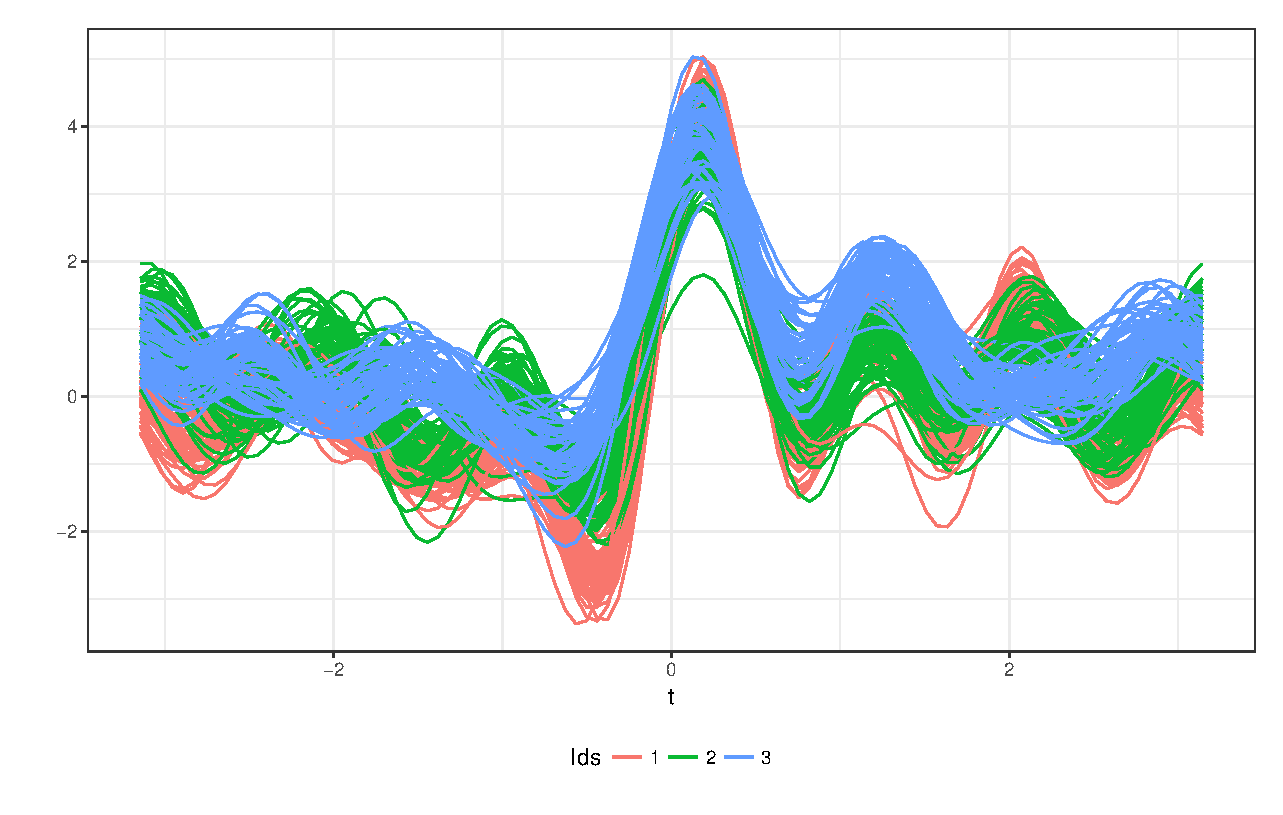
\includegraphics[width = 0.7\textwidth]{kmr.eps}
			\caption{K-means clustering result with random initialization, K = 3}
			\label{kmr}
		\end{figure}

		\item 
		Model based clustering:

		We use BIC to pick the model and number of clusters. In Figure~\ref{bic} we can see, model VVE and 3 clusters is the best. The display of clustering is shown in Figure~\ref{mcl_cl}. It is not easy to see, so we also displayed the result using \verb|ggandrews| as in (a) and (b) in Figure~.

		\begin{rcode}
# model based clustering
library(mclust)
mcl <- Mclust(wine.sc)
plot(mcl$BIC)
plot.Mclust(mcl, what = "classification")

# display using ggandrews
ggandrews(data.frame(mcl$classification, wine.sc), clr = 1, return_value = F)
		\end{rcode}

		\begin{figure}[!htb]
			\centering
			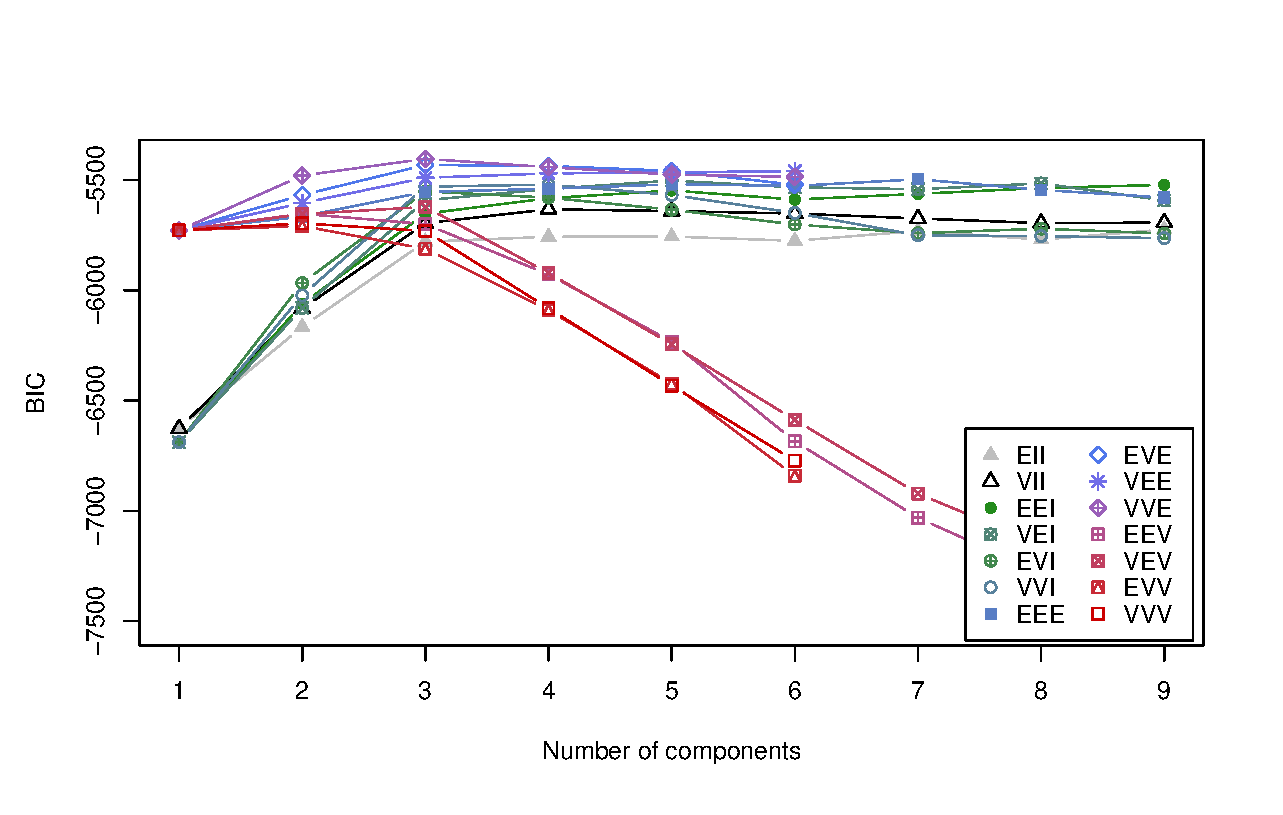
\includegraphics[width = 0.7\textwidth]{bic.eps}
			\caption{Model selection with BIC}
			\label{bic}
		\end{figure}
	\end{enumerate}

	\begin{figure}[!htb]
		\centering
		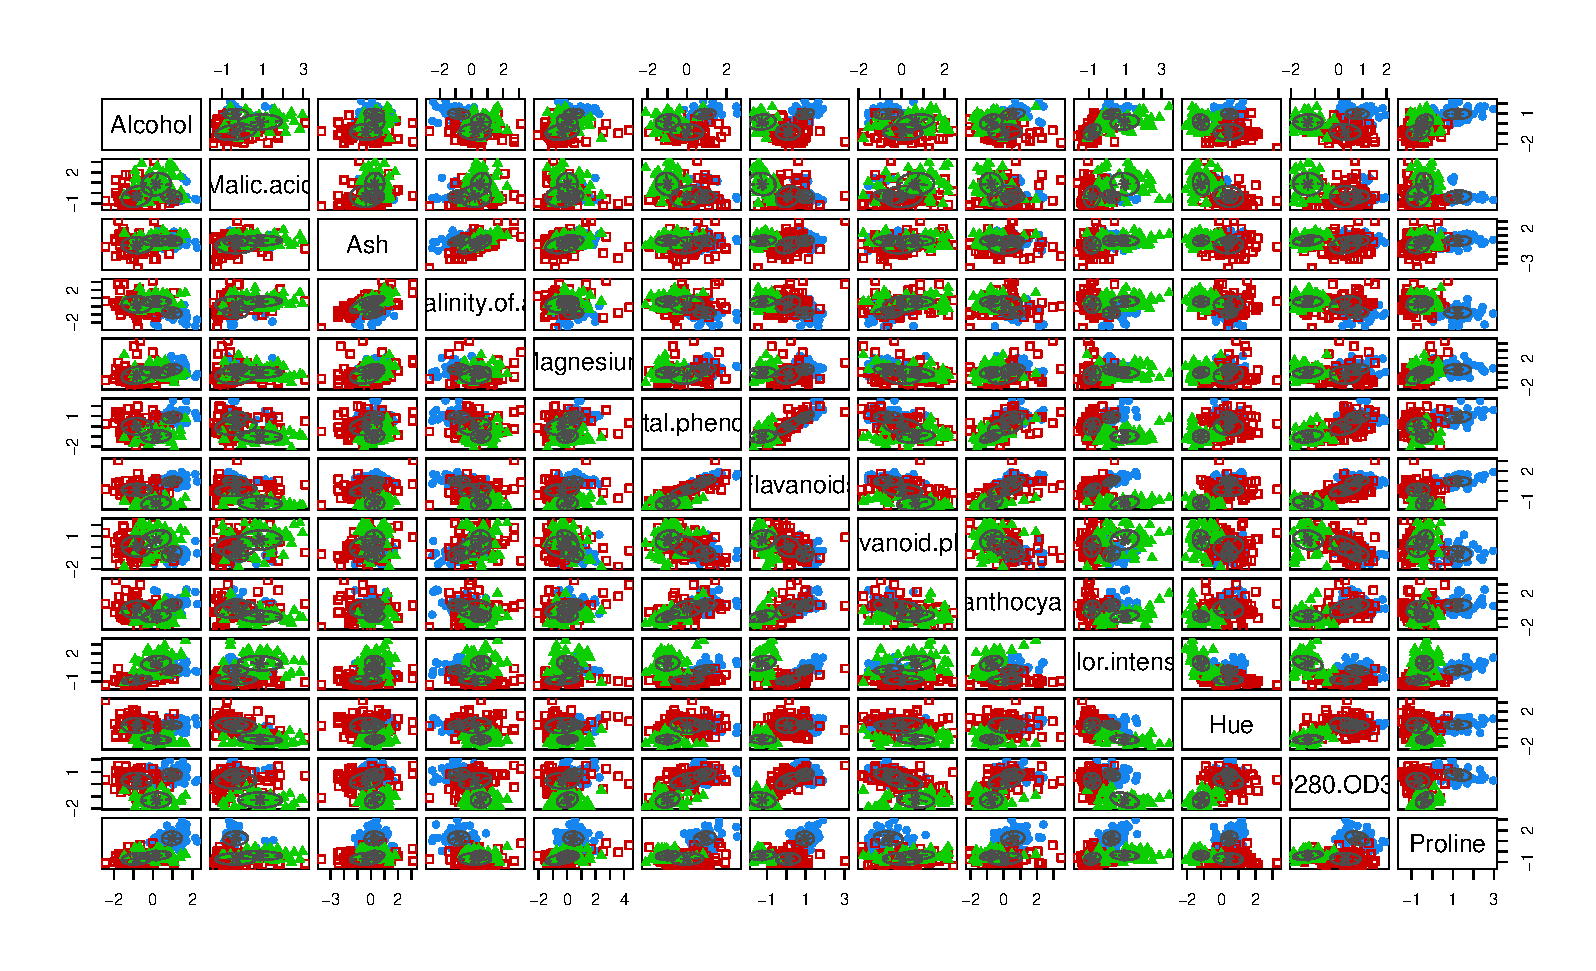
\includegraphics[width = 0.7\textwidth]{mcl_classification.eps}
		\caption{Model based clustering result, K = 3}
		\label{mcl_cl}
	\end{figure}

		\begin{figure}[!htb]
		\centering
		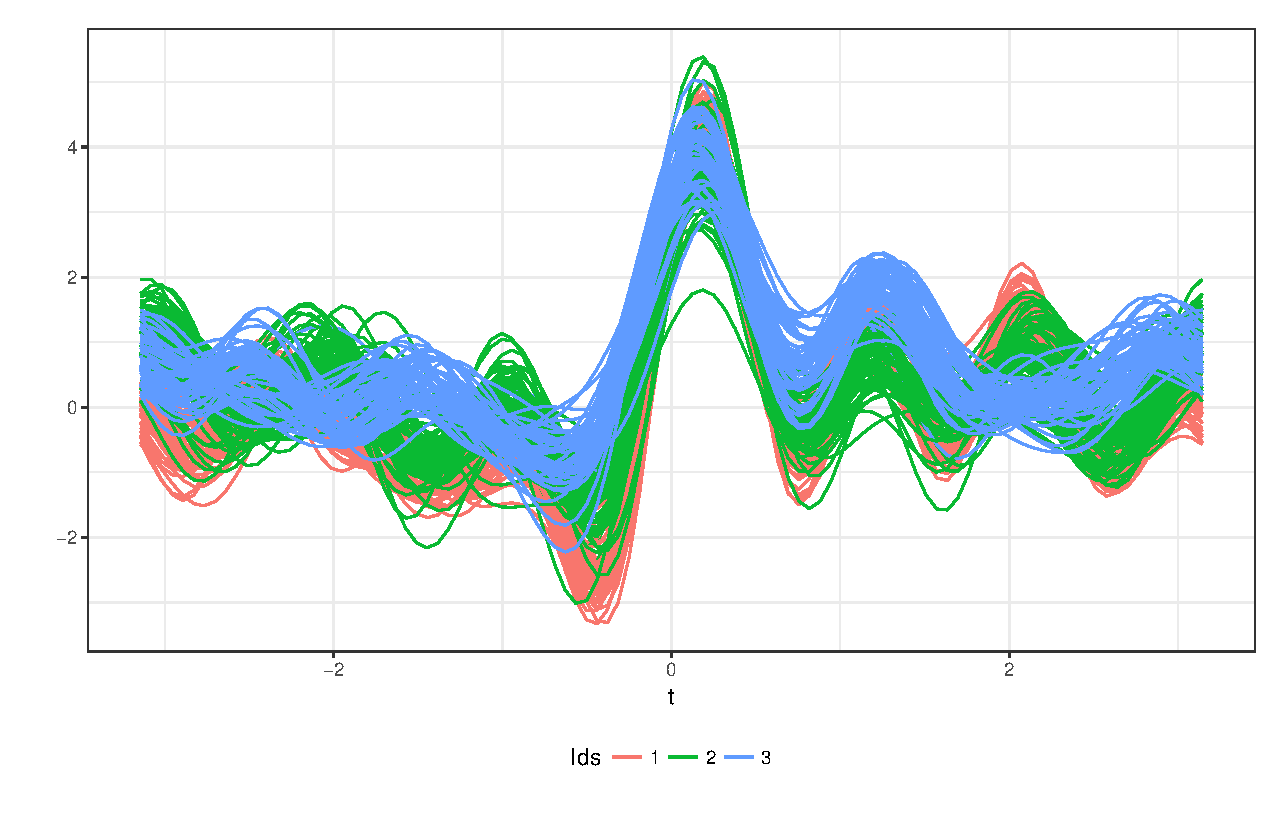
\includegraphics[width = 0.7\textwidth]{mcl.eps}
		\caption{Model based clustering result, K = 3}
		\label{mcl}
	\end{figure}

From the display, we can see the result of K-means (both initializations) and model based clustering are similar, and $K = 3$ is quite reasonable from the result. The result of hierarchical clustering is different and it seems like there is only one cluster in the final result. 

We then compare the clustering result with cultivar information with cross table of frequencies. 
\begin{rcode}
# compare the results with cultivar information
# hierarchical clustering with average linkage
ftable(table(cultivar, cutree(hc, k = 3)))

           1  2  3
cultivar          
1         58  1  0
2         68  2  1
3         48  0  0

# k-means innitialized with hc
ftable(table(cultivar, mapvalues(km$cluster, from = c(2,3,1), c(1,2,3))))

           1  2  3
cultivar          
1         59  0  0
2          3 65  3
3          0  0 48

# k-means with random initialization
ftable(table(cultivar, km.r$cluster))

           1  2  3
cultivar          
1         59  0  0
2          3 65  3
3          0  0 48

# model based clustering
ftable(table(cultivar, mcl$classification))

           1  2  3
cultivar          
1         56  3  0
2          0 70  1
3          0  0 48
\end{rcode}

We can see K-means and model based clustering gives the clusters that match the cultivar information very well (in K-means with hierarical clustering initilization, we renamed the clusters to match the cultivar information). And the result of hierarchical clustering is not good. It clustered almost all observations to one cultivar.  

\item 
We use the standardized data to perform PCA.
\begin{rcode}
# PCA
wine.pc <- prcomp(wine.sc)
#  compute proportion of total variance explained by 
#  each component

s <- wine.pc$sdev^2                                

pvar<-s/sum(s)
cat("proportion of variance: ", pvar, fill=T) 

#  cumulative proportion of total variance explained 
#  by each component

cpvar <- cumsum(s)/sum(s)
cat("cumulative proportion of variance: ", cpvar, fill=T)
\end{rcode}
The proportion is variance and cumulative proportion of variance are:
\begin{rcode}
proportion of variance:  0.3619885 0.1920749 0.1112363 0.0706903 0.06563294 0.04935823 0.04238679 0.02680749 0.02222153 
0.01930019 0.01736836 0.01298233 0.007952149

cumulative proportion of variance:  0.3619885 0.5540634 0.6652997 0.73599 0.8016229 0.8509812 0.893368 0.9201754 
0.942397 0.9616972 0.9790655 0.9920479 1
\end{rcode}

Based on the cumulative proportion of variance, we then test for 4 and 5 PCs for explaining 80\% of total variance.
\begin{rcode}
# test 5 is enough while 4 is not
source("PCs.proportion.variation.enuff.R")
PCs.proportion.variation.enuff(lambda = s, q = 4, nobs = nrow(wine.sc), propn = 0.8)
PCs.proportion.variation.enuff(lambda = s, q = 5, nobs = nrow(wine.sc), propn = 0.8)
\end{rcode}

The p-values are 0 and 1 respectively. So we conclude that the first 5 PCs are enough to explain 80\% of variance in the data. 

The first 5 PCs are:
\begin{rcode}
# first 5 PCs
wine.pc$rotation[,1:5]

                              PC1          PC2         PC3         PC4         PC5
Alcohol              -0.144329395  0.483651548 -0.20738262  0.01785630 -0.26566365
Malic.acid            0.245187580  0.224930935  0.08901289 -0.53689028  0.03521363
Ash                   0.002051061  0.316068814  0.62622390  0.21417556 -0.14302547
Alkalinity.of.ash     0.239320405 -0.010590502  0.61208035 -0.06085941  0.06610294
Magnesium            -0.141992042  0.299634003  0.13075693  0.35179658  0.72704851
Total.phenols        -0.394660845  0.065039512  0.14617896 -0.19806835 -0.14931841
Flavanoids           -0.422934297 -0.003359812  0.15068190 -0.15229479 -0.10902584
Nonflavanoid.phenols  0.298533103  0.028779488  0.17036816  0.20330102 -0.50070298
Proanthocyanins      -0.313429488  0.039301722  0.14945431 -0.39905653  0.13685982
Color.intensity       0.088616705  0.529995672 -0.13730621 -0.06592568 -0.07643678
Hue                  -0.296714564 -0.279235148  0.08522192  0.42777141 -0.17361452
OD280.OD315          -0.376167411 -0.164496193  0.16600459 -0.18412074 -0.10116099
Proline              -0.286752227  0.364902832 -0.12674592  0.23207086 -0.15786880
\end{rcode}

Each of the 5 PCs seems like contrast of these 13 measures. For example, the firt PC is the difference of weighted mean of malic acid, ash, alkalinity of ash, nonflavanoid phenols and color intensity between the weighted mean of alcohol, magnesium, total phenols, flavanoids, proanthocyains, hue, OD280/OD315 and proline. The rest can also be interpreted in this way.


 \item 
 We first split the data into training set and test set.
 \begin{rcode}
 # split data
set.seed(8413)
train.idx <- sample(1:nrow(wine), size = 128, replace = F)
wine.train <- wine[train.idx,]
wine.test <- wine[-train.idx,]
  \end{rcode} 

  Then for each method, we calculate the AER and LOOCV misclassification rate in training set and also the misclassification rate in test set with the classification rule trained with training set.

\begin{enumerate}
	\item
	QDA:
\begin{rcode}
# QDA
library(MASS)
wine.qda <- qda(Cultivar ~ ., data = wine.train, CV = F)

# AER
mean(wine.train$Cultivar!=predict(wine.qda)$class) 

# CV
wine.qda.cv <- qda(Cultivar ~ ., data = wine.train, CV = T)
mean(wine.train$Cultivar!=wine.qda.cv$class) 

# misclassification on test set
mean(wine.test$Cultivar!=predict(wine.qda, newdata = wine.test[,-1])$class)
\end{rcode}
The result of QDA:
\begin{align*}
&\mathrm{AER} = 0\\
&\mathrm{LOOCV} = 0.0078125\\
& \mathrm{test} = 0 
\end{align*}

\item 
k-NN:

We first find the optimal $k$ among $\{1,2,\ldots, 10\}$ with leave-one-out cross-validation (function \verb|knn.cv| is used). The cross valication error rate for each $k$ is shown in Figure~\ref{knn}. From Figure~\ref{knn} we can see $k = 5$ is the optimal one, and we use $k = 5$ to calculate our misclassifivation rates.
\begin{rcode}
#kNN
library(class)
# using cross-validation to pick k
# using scaled data
wine.train.sc <- scale(wine.train[,-1])
wine.test.sc <- scale(wine.test[,-1])
# try k = 1,..,10
knn.cv.err<-NULL
knn.cv.sd<-NULL
for (i in 1:10) { 
  temp<-NULL
  for (j in 1:10000)
    temp <- c(temp,mean(knn.cv(wine.train.sc,
                               cl = wine.train$Cultivar, k = i) != wine.train$Cultivar))
  knn.cv.err<-c(knn.cv.err,mean(temp))
  knn.cv.sd<-c(knn.cv.sd,sd(temp))
  cat("\n Done i= ",i)
}


plot(knn.cv.err, xlim = c(1, 10),
     ylim=c(min(knn.cv.err - 1.96 * knn.cv.sd),
            max(knn.cv.err + 1.96 * knn.cv.sd)), type = "n")
lines(knn.cv.err + 1.96 * knn.cv.sd, lty = 2, col = "blue")
lines(knn.cv.err - 1.96 * knn.cv.sd, lty = 2, col = "green")
lines(knn.cv.err, col = "red")

# use k = 5

wine.knn.train <- knn(train = wine.train.sc, test = wine.train.sc, cl = wine.train$Cultivar, k = 5)

#AER
mean(wine.knn.train != wine.train$Cultivar)

#CV
knn.cv.err[5]

# misclassification on test set
wine.knn <- knn(train = wine.train.sc, test = wine.test.sc, cl = wine.train$Cultivar, k = 5)
mean(wine.knn != wine.test$Cultivar)
\end{rcode}

\begin{figure}[!htb]
	\centering
	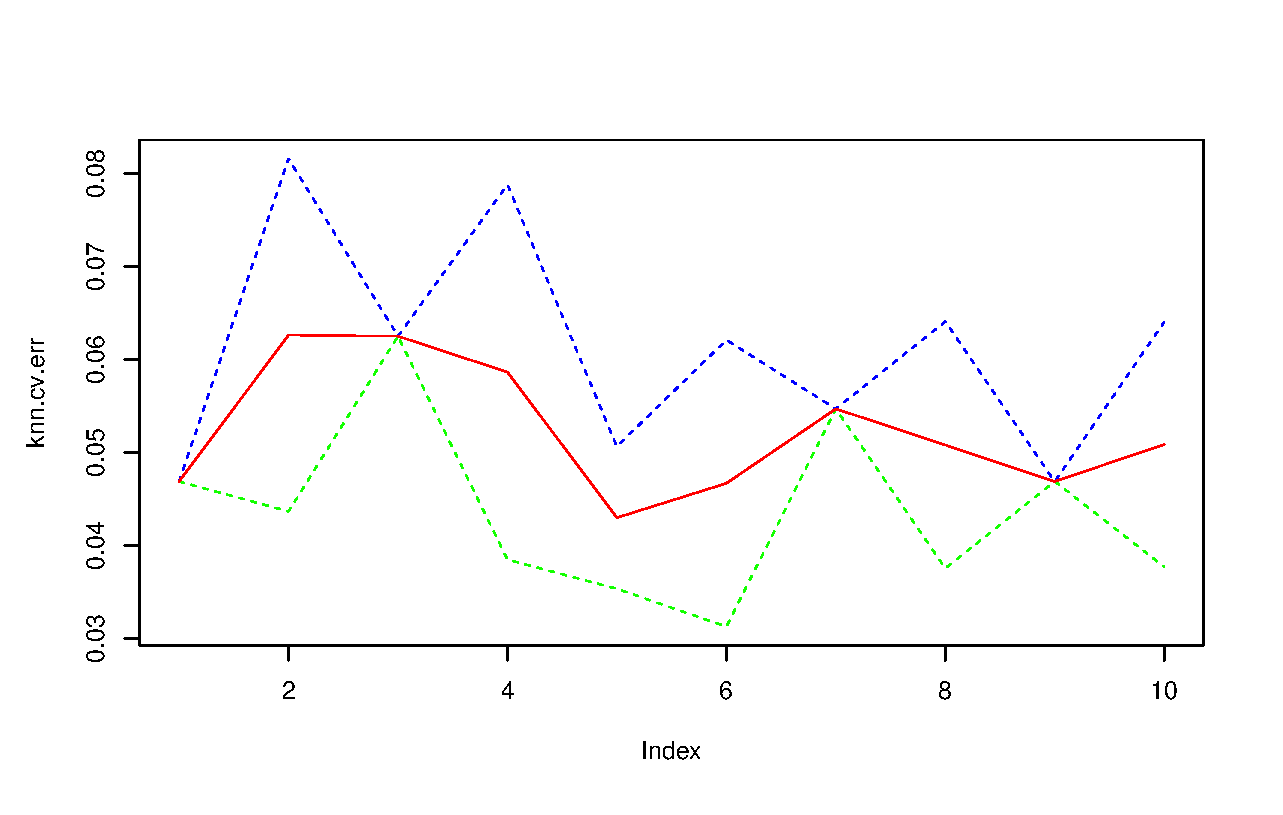
\includegraphics[width = 0.7\textwidth]{knncv.eps}
	\caption{Finding the optimal $k$ for k-NN}
	\label{knn}
\end{figure}

The result of k-NN:
\begin{align*}
&\mathrm{AER} = 0.03125\\
&\mathrm{LOOCV} = 0.04298281\\
& \mathrm{test} = 0.06
\end{align*}

\item 
CART:

We first find the optimal tree with leave-one-out cross-validation (function \verb|cv.tree| is used). From Figure~\ref{findtree} we can see when number of nodes is 4, we got the optimal tree (Figure!\ref{opttree}). Then we calculated misclassification rates with this tree. 
\begin{rcode}
# CART
library(tree)
# getting optimal tree using cross-validation
wine.tree <- tree(formula = Cultivar ~ ., data = wine.train)
wine.tree.cv <- cv.tree(wine.tree, K = nrow(wine.train))
plot(wine.tree.cv)
# the best one is 4. Plot the best one.
wine.tree.opt <- prune.tree(wine.tree, k = 4)
plot(wine.tree.opt)
text(wine.tree.opt)

#AER 
mean(apply(predict(wine.tree.opt), 1, which.max)!=wine.train$Cultivar)

#CV
mean(sapply(1:nrow(wine.train), function(x) mean(mean(apply(predict(tree(Cultivar ~ ., data = wine.train[-x,]), newdata = wine.train[,-1]), 1, which.max)!=wine.train$Cultivar))))

# misclassification on test set
mean(apply(predict(wine.tree.opt, newdata = wine.test[,-1]), 1, which.max)!=wine.test$Cultivar) 
\end{rcode}

\begin{figure}[!htb]
	\centering
	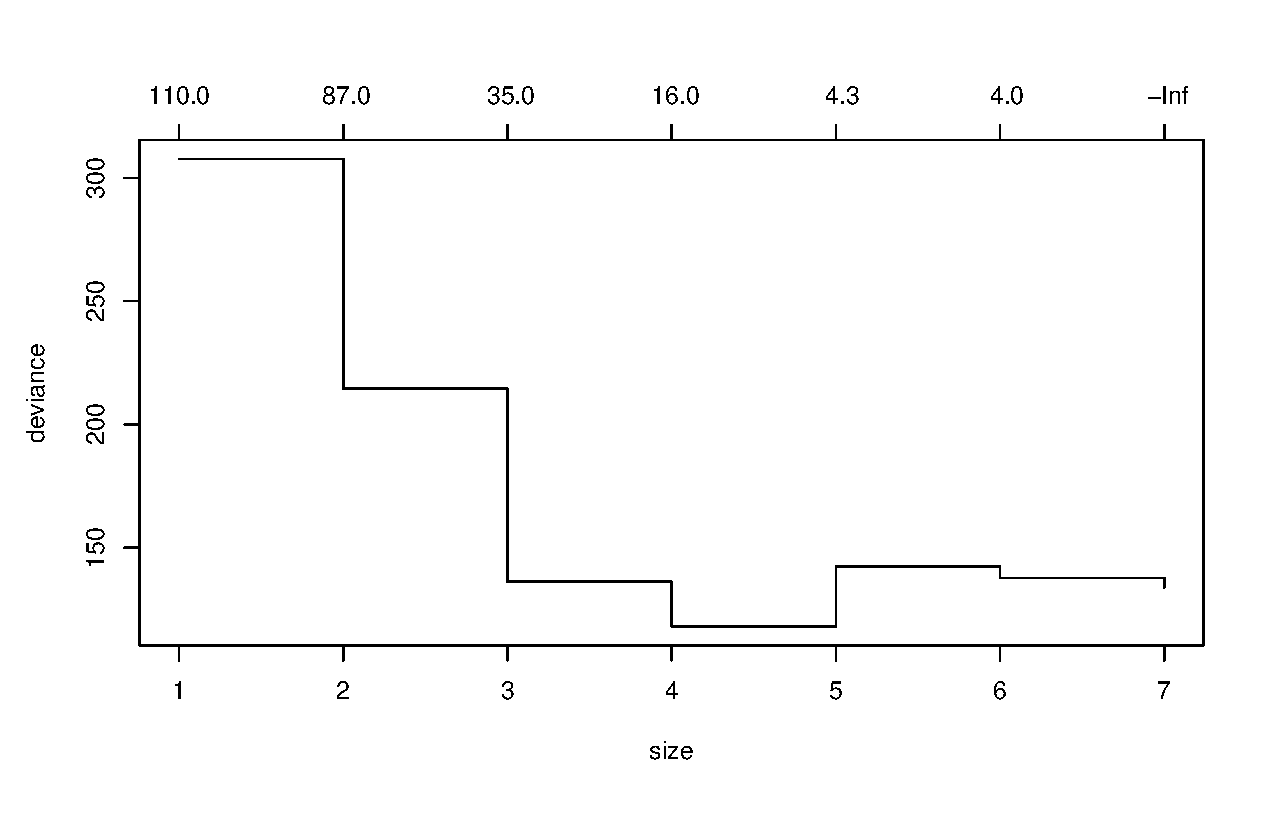
\includegraphics[width = 0.7\textwidth]{findtree.eps}
	\caption{Finding the optimal tree}
	\label{findtree}
\end{figure}

\begin{figure}[!htb]
	\centering
	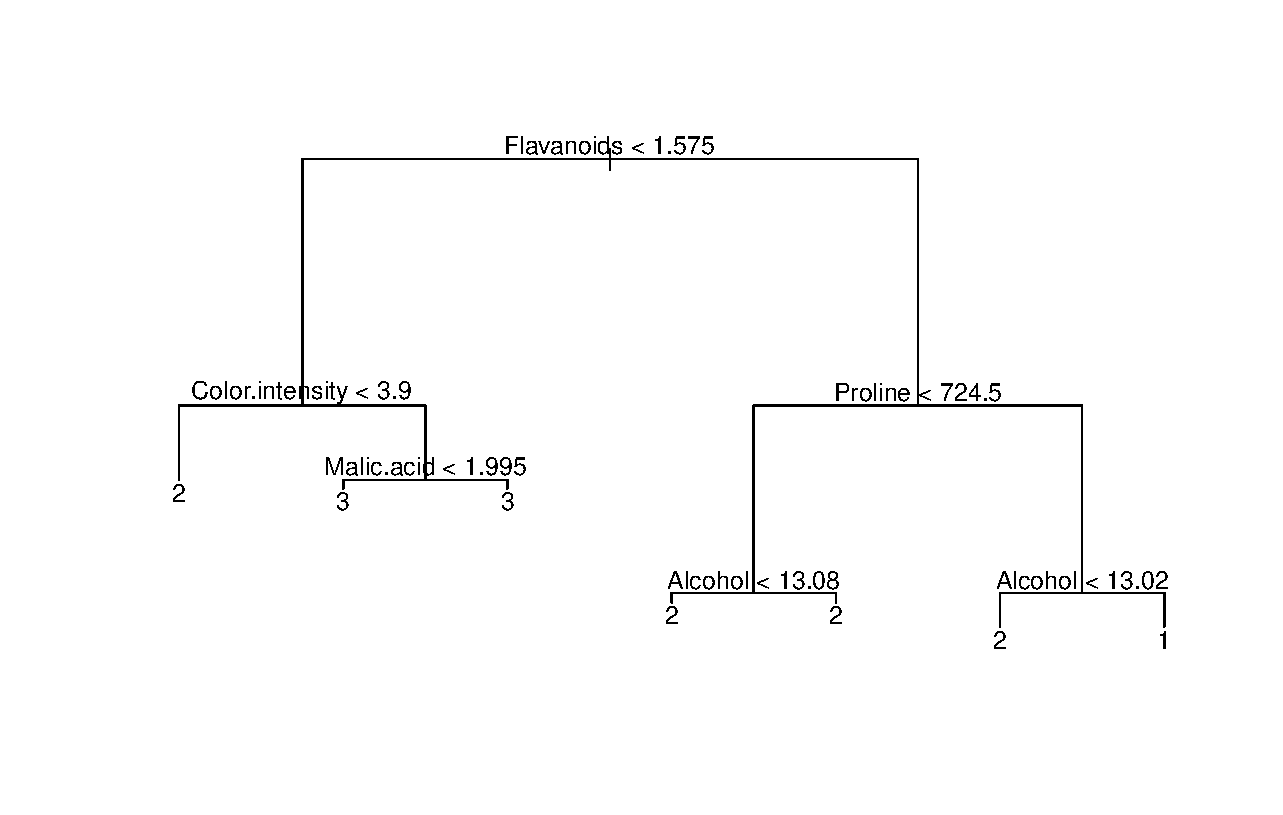
\includegraphics[width = 0.7\textwidth]{opttree.eps}
	\caption{Optimal tree, k = 4}
	\label{opttree}
\end{figure}

The result of CART:
\begin{align*}
&\mathrm{AER} = 0.03125\\
&\mathrm{LOOCV} = 0.03167725\\
& \mathrm{test} = 0.02
\end{align*}
\end{enumerate}

Now we summarise the missclassification rates in the Table~\ref{miscr} below. From the table, we can see that QDA gives the smallest misclassification rates in AER, LOOCV and test. Thus for this data set, we can use QDA as a classification rule as it out-performs others.

\begin{table}
\caption{Summary of missclassification rates}
\label{miscr}
\begin{center}
\begin{tabular}{cccc}
\toprule
  & QDA & k-NN & CART \\
  \midrule
AER & 0 &  0.03125 & 0.03125\\
LOOVA &  0.0078125 & 0.04298281 & 0.03167725\\
test & 0 & 0.06 & 0.02\\
\bottomrule
\end{tabular}\end{center}
\end{table}

\newpage
\item
We display the first 5 PCs using 2D and 3D radial visualization in Figure~\ref{2drad} and Figure~\ref{3drad}. The cultivars are distinguishable in both 2D and 3D radial visualization, but we can see less overlapping with the 3D radial visualization (a specific angle of view was picked here in Figure~\ref{3drad} to show the non-overlapping of 3 cultivars).
\begin{rcode}
# display the first 5 PCs using 3d radviz
source("radviz3d-3.R")
radialvis3d(data = wine.pc$x[,1:5], cl = wine$Cultivar)
rgl.snapshot("radviz3d.jpg")
# using 2d radviz
source("radviz2d.R")
source("mmnorm.R")
source("circledraw.R")
radviz2d(dataset = cbind(wine.pc$x[,1:5], wine$Cultivar), name = "wine")
\end{rcode}

\begin{figure}[!htb]
	\centering
	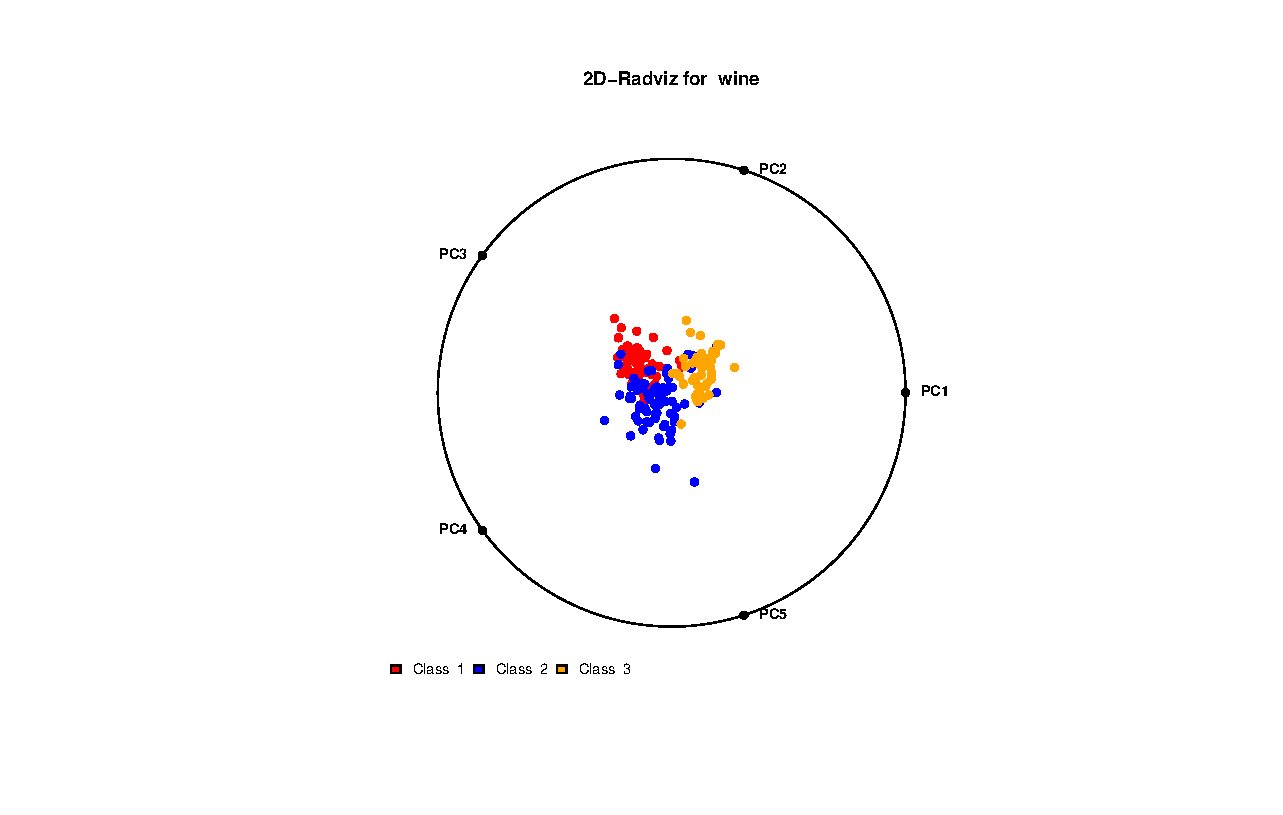
\includegraphics[width = \textwidth]{radviz2d.eps}
	\caption{2D radial visualization}
	\label{2drad}
\end{figure}

\begin{figure}[!htb]
	\centering
	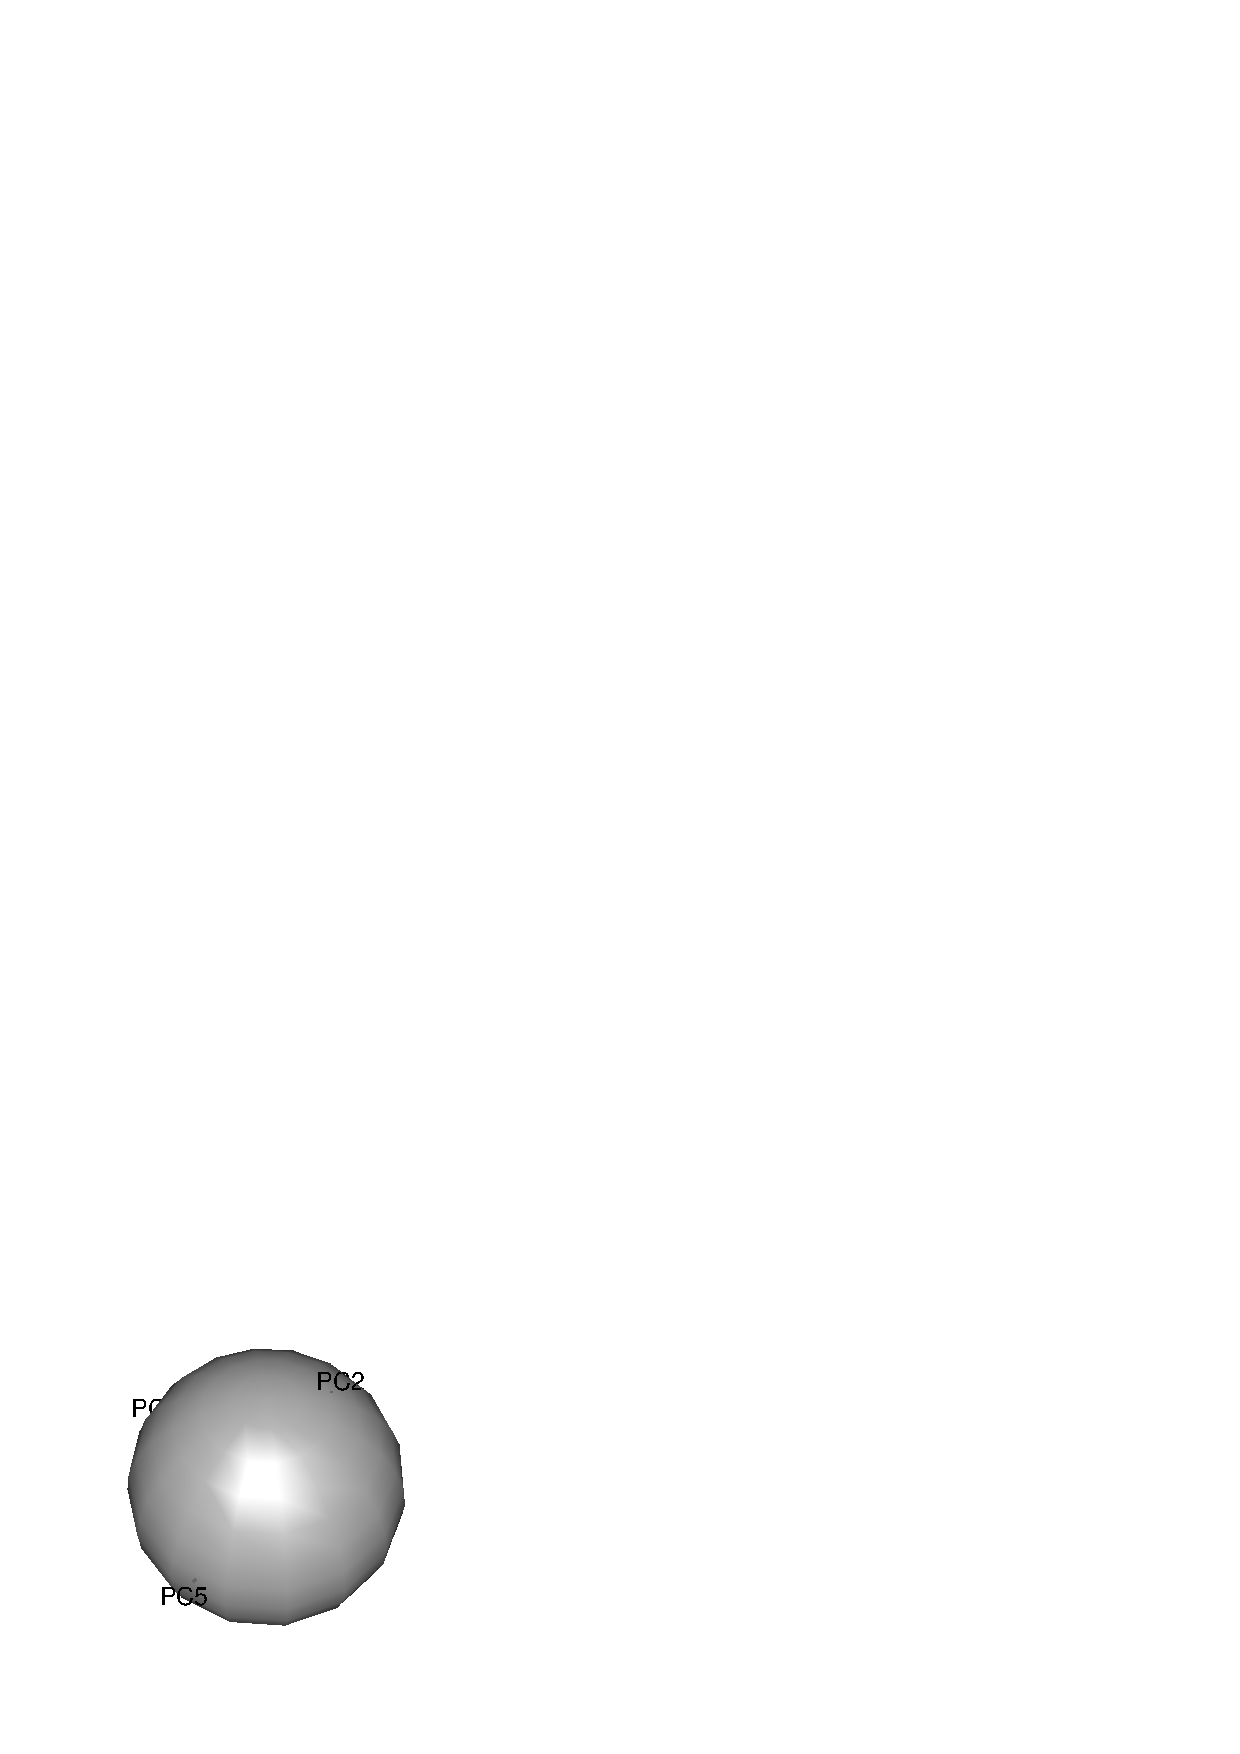
\includegraphics[width = 0.7\textwidth]{radviz3d.png}
	\caption{3D radial visualization}
	\label{3drad}
\end{figure}
 \end{enumerate}











	
	
	
	\end{document}